
% \documentclass[12pt]{article}
\documentclass[10pt]{scrartcl}
\title{Algebra I}
\nonstopmode
%\usepackage[utf-8]{inputenc}
\usepackage{graphicx} % Required for including pictures
% \usepackage[figurename=Figure]{caption}
\usepackage{verbatim} % For comments and other
\usepackage{amsmath}  % For math
\usepackage{amssymb}  % For more math
\usepackage{fullpage} % Set margins and place page numbers at bottom center
\usepackage{paralist} % paragraph spacing
\usepackage{listings} % For source code
\usepackage{libertine}
\usepackage{array,epsfig}
\usepackage{amsfonts}
\usepackage{amssymb}
\usepackage{amsxtra}
\usepackage{amsthm}
\usepackage{mathrsfs}
\usepackage{color}
\usepackage{stmaryrd}
\usepackage{microtype}
\usepackage{aligned-overset}
\usepackage{wrapfig}
\usepackage{subcaption}
%\usepackage[russian,english]{babel}

\setlength{\parindent}{0pt}

\renewcommand*{\proofname}{Beweis}

\newcommand{\lra}{\longrightarrow}
\newcommand{\ra}{\rightarrow}
\newcommand{\la}{\leftarrow}
\newcommand{\surj}{\twoheadrightarrow}
\newcommand{\graph}{\mathrm{graph}}
\newcommand{\bb}[1]{\mathbb{#1}}
\newcommand{\Z}{\bb{Z}}
\newcommand{\Q}{\bb{Q}}
\newcommand{\R}{\bb{R}}
\newcommand{\CC}{\bb{C}}
\newcommand{\N}{\bb{N}}
\newcommand{\M}{\mathbf{M}}
\newcommand{\MM}{\mathscr{M}}
\newcommand{\HH}{\mathscr{H}}
\newcommand{\Om}{\Omega}
\newcommand{\Ho}{\in\HH(\Om)}
\newcommand{\bd}{\partial}
\newcommand{\del}{\partial}
\newcommand{\bardel}{\overline\partial}
\newcommand{\textdf}[1]{\textbf{\textsf{#1}}\index{#1}}
\newcommand{\img}{\mathrm{img}}
\newcommand{\ip}[2]{\left\langle{#1},{#2}\right\rangle}
\newcommand{\inter}[1]{\mathrm{int}{#1}}
\newcommand{\exter}[1]{\mathrm{ext}{#1}}
\newcommand{\cl}[1]{\mathrm{cl}{#1}}
\newcommand{\ds}{\displaystyle}
\newcommand{\vol}{\mathrm{vol}}
\newcommand{\cnt}{\mathrm{ct}}
\newcommand{\osc}{\mathrm{osc}}
\newcommand{\LL}{\mathbf{L}}
\newcommand{\UU}{\mathbf{U}}
\newcommand{\support}{\mathrm{support}}
\newcommand{\AND}{\;\wedge\;}
\newcommand{\OR}{\;\vee\;}
\newcommand{\Oset}{\varnothing}
\newcommand{\st}{\ni}
\newcommand{\wh}{\widehat}
\newcommand{\zz}[1]{Z\kern-.3em\raise-0.5ex\hbox{Z} : #1}%Zu zeigen symbol
\newcommand{\vereinigung}{\cup}
\newcommand{\schnitt}{\cap}
\newcommand{\m}{\cdot} % use \m for mulitplication dot
\newcommand{\limes}[1]{\underset{#1}{\lim}} % use \limes{r \to \infty} for underset limit
\newcommand{\widerspruch}{\lightning}
\newcommand{\sub}[1]{\subsection*{#1)}}
\newcommand{\subsub}[1]{\subsubsection*{#1.}}
\newcommand{\auf}[1]{\paragraph*{Aufgabe #1}}
\newcommand{\beschriftetesistgleich}[1]{\overset{\text{#1}}{=}}
\newcommand{\ue}[1]{\underset{\text{#1}}{=}}
\newcommand{\mng}[1]{\left\{#1\right\}} % autoscaling curly braces
\newcommand{\parenth}[1]{\left(#1\right)} % autoscaling parentheses
\newcommand{\squarebr}[1]{\left[#1\right]} % autoscaling squarebrackets
\newcommand{\spn}[1]{\left\langle#1\right\rangle} % autoscaling span brackets
\newcommand{\abs}[1]{\left|#1\right|} % autoscaling absolute symbol
\newcommand{\norm}[1]{\left\Vert#1\right\Vert} % autoscaling norm symbol
\newcommand{\frk}[1]{\mathfrak{#1}}
\newcommand{\mc}[1]{\mathcal{#1}}
\newcommand{\eps}{\varepsilon}
\newcommand{\E}{\mathbb{E}}
\newcommand{\V}{\mathbb{V}}
\newcommand{\ent}{\text{Ent}}
\newcommand{\id}{1\hspace{-0,9ex}1}
\newcommand{\1}{1\hspace{-0,9ex}1}
\newcommand{\Prb}{\mathbb{P}}

\begin{document}

\begin{center}
	\hrule
	\vspace{.4cm}
	{\large PRAKTIKUM NUMERIK}
\end{center}
{\textbf{Name:}\ Mikael Lux \& Ulf Gerking\hspace{\fill} \textbf{Abgabedatum:} tbd}\\
{ \textbf{Matrikelnummern:}} \ 3704083  \& 3739341 \hspace{\fill} \\
\hrule
\section*{Einleitung}
Im folgendem werden wir unsere Implementationen einiger Algorithmen zum lösen nicht-linearer Gleichungen vorstellen und unter Zuhilfenahme einiger Diagramme auswerten. Genauer gesagt soll für diverse Funktionen $f:[0,1] \to \R$ eine Lösung $x^*\in[0,1]$ mit $f(x^*)=0$ gefunden werden.
\section*{Verwendete Algorithmen}
\subsection*{Newton-Verfahren}
Beim Newton Verfahren wählen wir einen Startwert $x_0\in[0,1]$ und nähern uns der Lösung iterativ durch die Vorschrift
\[
	x_{n+1} = x_n + \frac{f(x_n)}{f'(x_n)}
\]
Dies entspricht dem Schnittpunkt der Tangente an $f$ durch $x_n$ und der $x$-Achse.
\begin{figure}[!h]
	\centering
	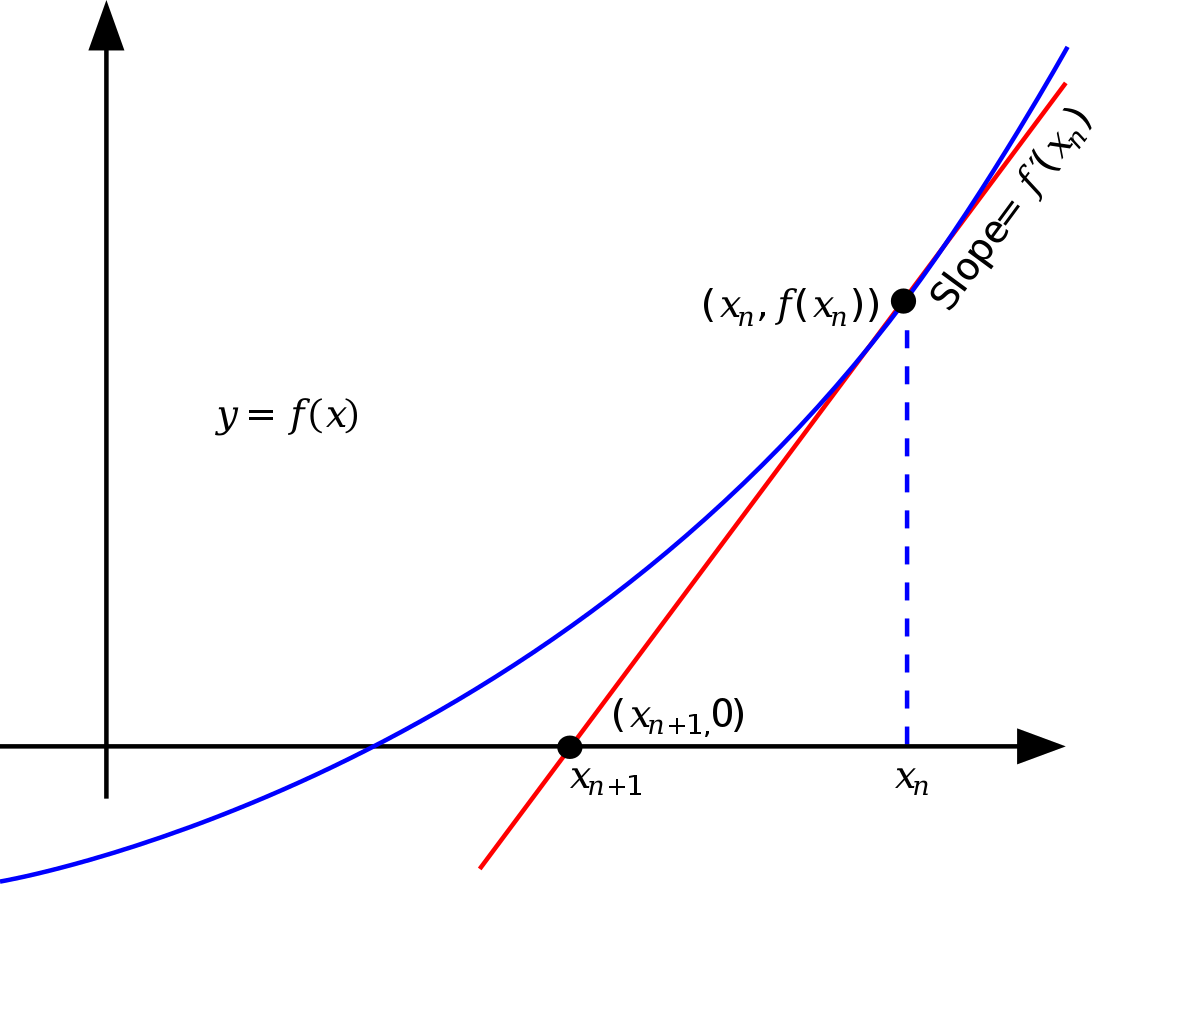
\includegraphics[width=0.75\textwidth]{plots/newtons_method.png}
	\caption{Veranschaulichung eines Iterationsschrittes des Newton-Verfahrens}
\end{figure}
\subsection*{Sekantenverfahren}
Für das Sekantenverfahren wählen wir zwei Anfangswerte $x_0,x_1 \in [0,1]$ und erhalten Näherungswerte durch
\[
	x_{n+1}= x_n - f(x_{n-1})\frac{x_{n-1}-x_{n-2}}{f(x_{n-1})-f(x_{n-2})}
\]
Es fällt sofort die Ähnlichkeit zum Newton-Verfahren auf, $f'$ wurde hier lediglich durch einen Differenzenquotienten ersetzt. Hier wählen wir also den Schnittpunkt der Sekanten durch $(x_{n-2}, f(x_{n-2}))$ und $(x_{n-1}, f(x_{n-1}))$ mit der $x$-Achse um den nächsten Näherungswert zu erhalten.
\begin{figure}[!h]
	\centering
	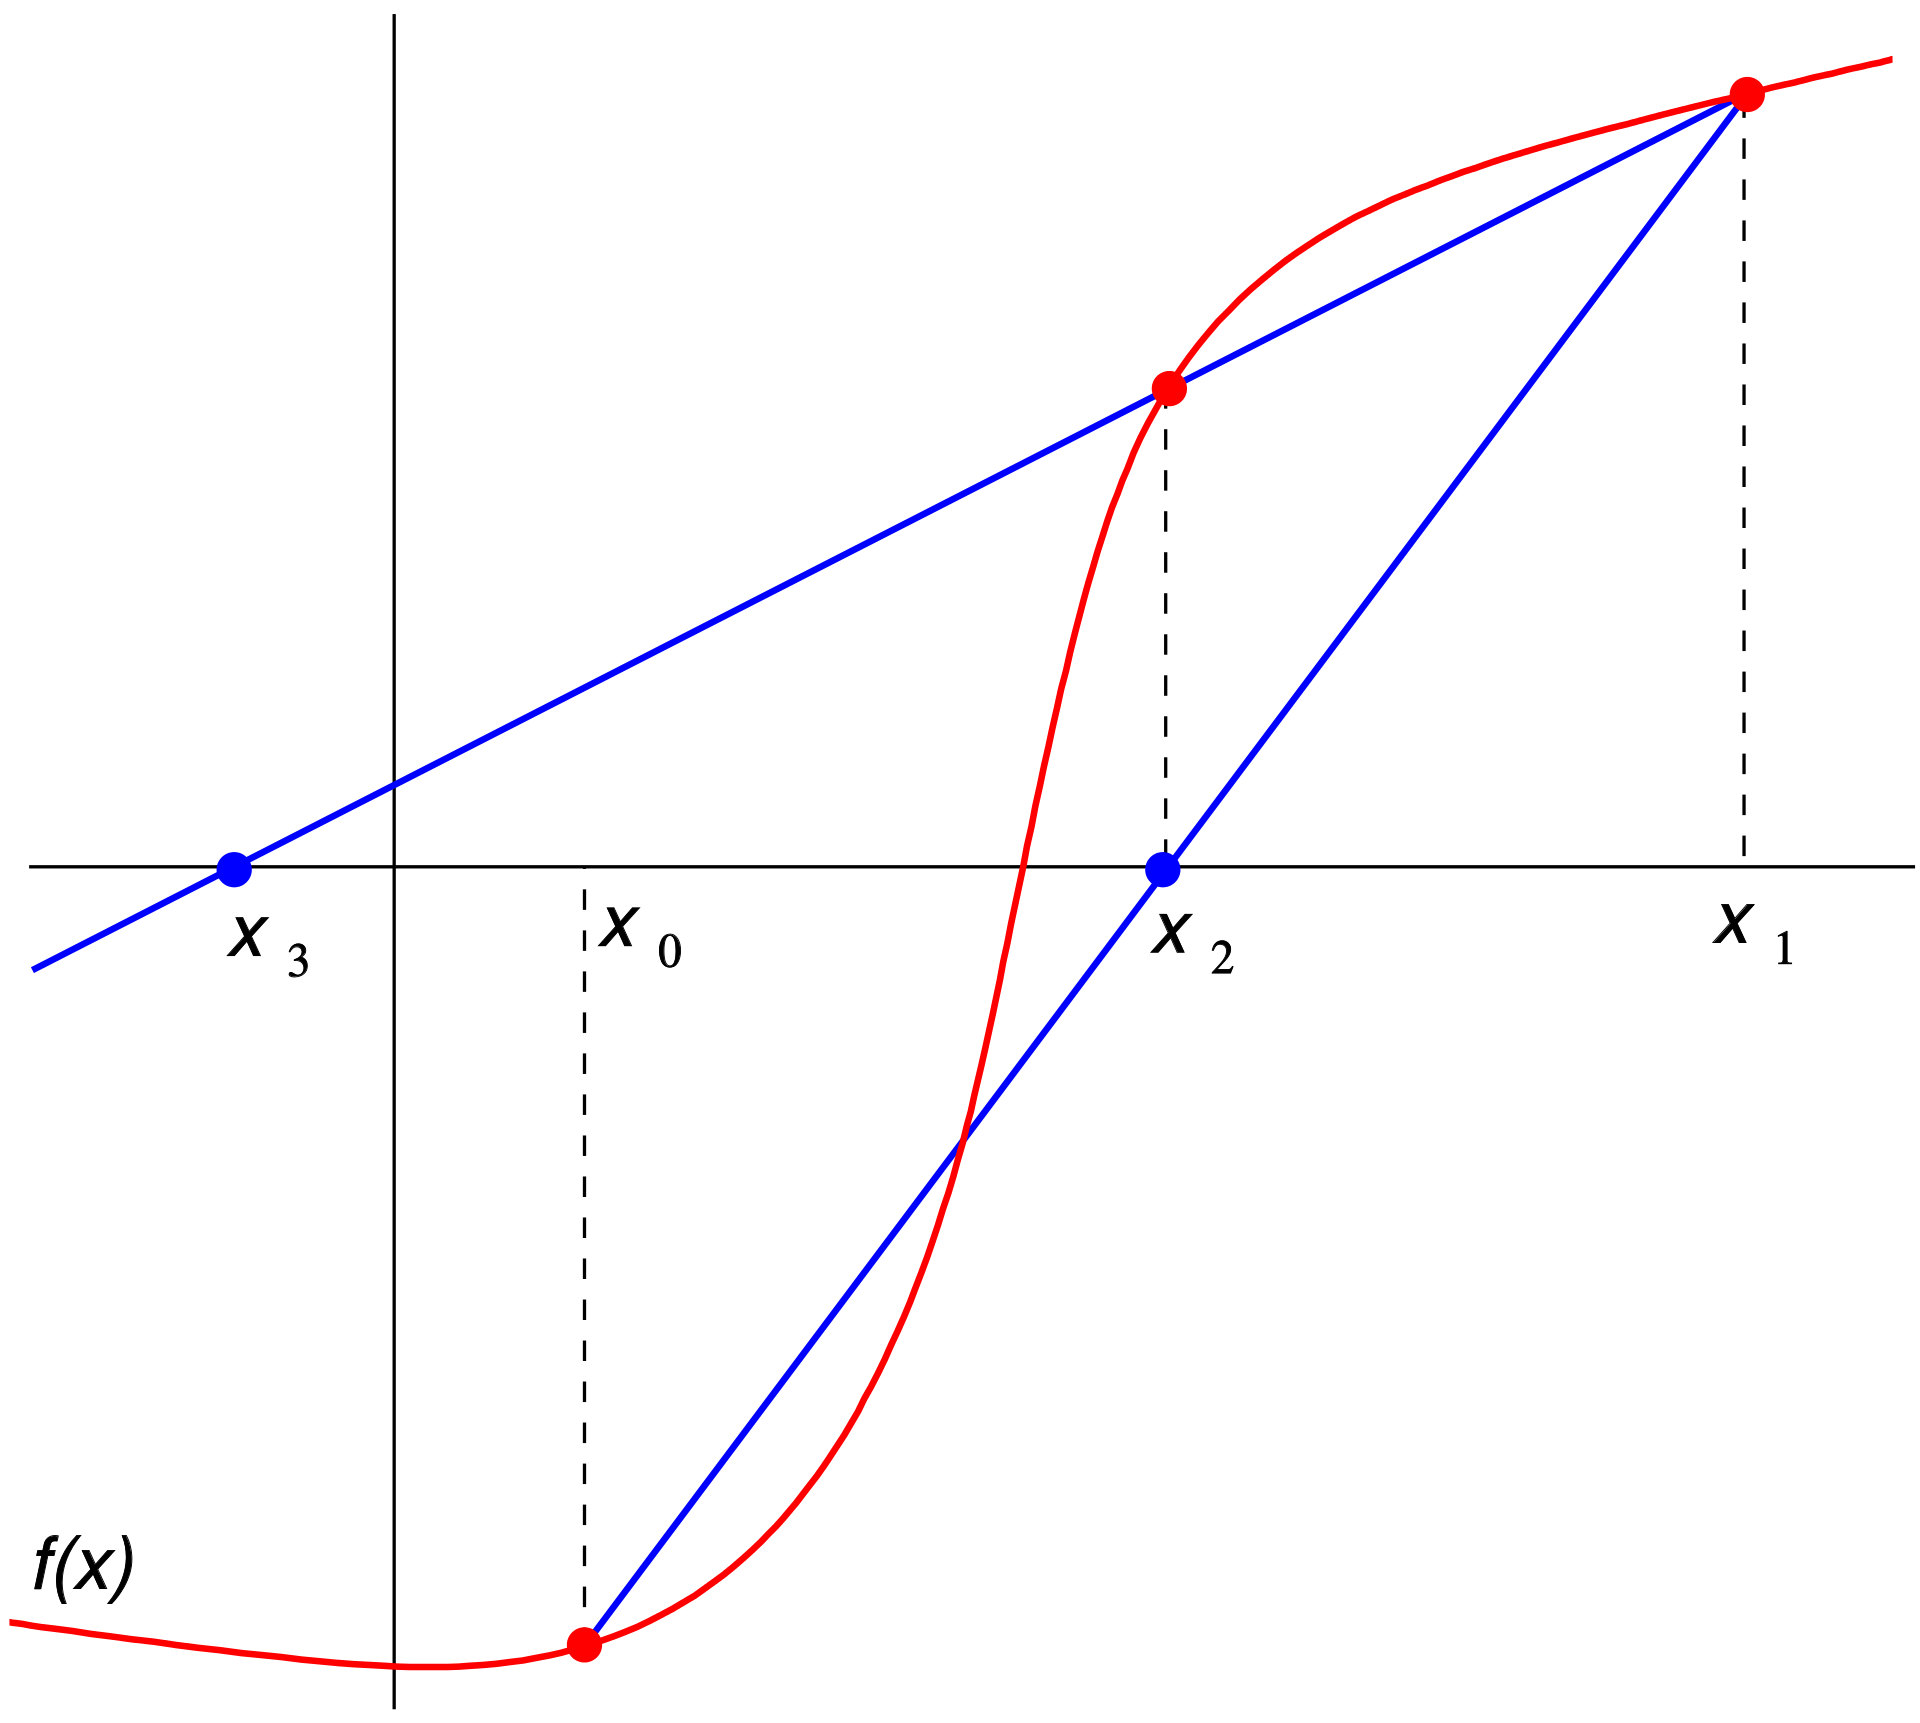
\includegraphics[width=0.75\textwidth]{plots/sekant.png}
	\caption{Veranschaulichung einiger Iterationsschritte des Sekantenverfahrens}
\end{figure}
\subsection*{Bisektionsverfahren}
Beim Bisektionsverfahren beginnen wir mit einem Startintervall $[a_0, b_0] \subseteq [0,1]$ mit $f(a_0)f(b_0) < 0$ (d.h. in diesem Intervall existiert eine Nullstelle). Wir betrachten in jedm Iterationsschritt nun den Mittelpunkt dieses Intervalles $x_n = \frac{a_n + b_n}{2}$, nun Überprüfen wir das Vorzeichen von $f, sgn(f(x_n))$ an dieser Stelle und Verkleinern das Intervall nach folgender Vorschrift:
\[
	a_{n+1} = \begin{cases}
		x_n\text{ falls} sgn(f(x_n))=sgn(f(a_n)), \\
		a_n\text{ sonst}
	\end{cases}, b_{n+1} = \begin{cases}
		x_n\text{ falls} sgn(f(x_n))=sgn(f(b_n)), \\
		b_n\text{ sonst}
	\end{cases}
\]
Dem Informatikaffinen Leser fällt vielleicht die ähnlichkeit zur binären Suche auf.
\begin{figure}[!h]
	\centering
	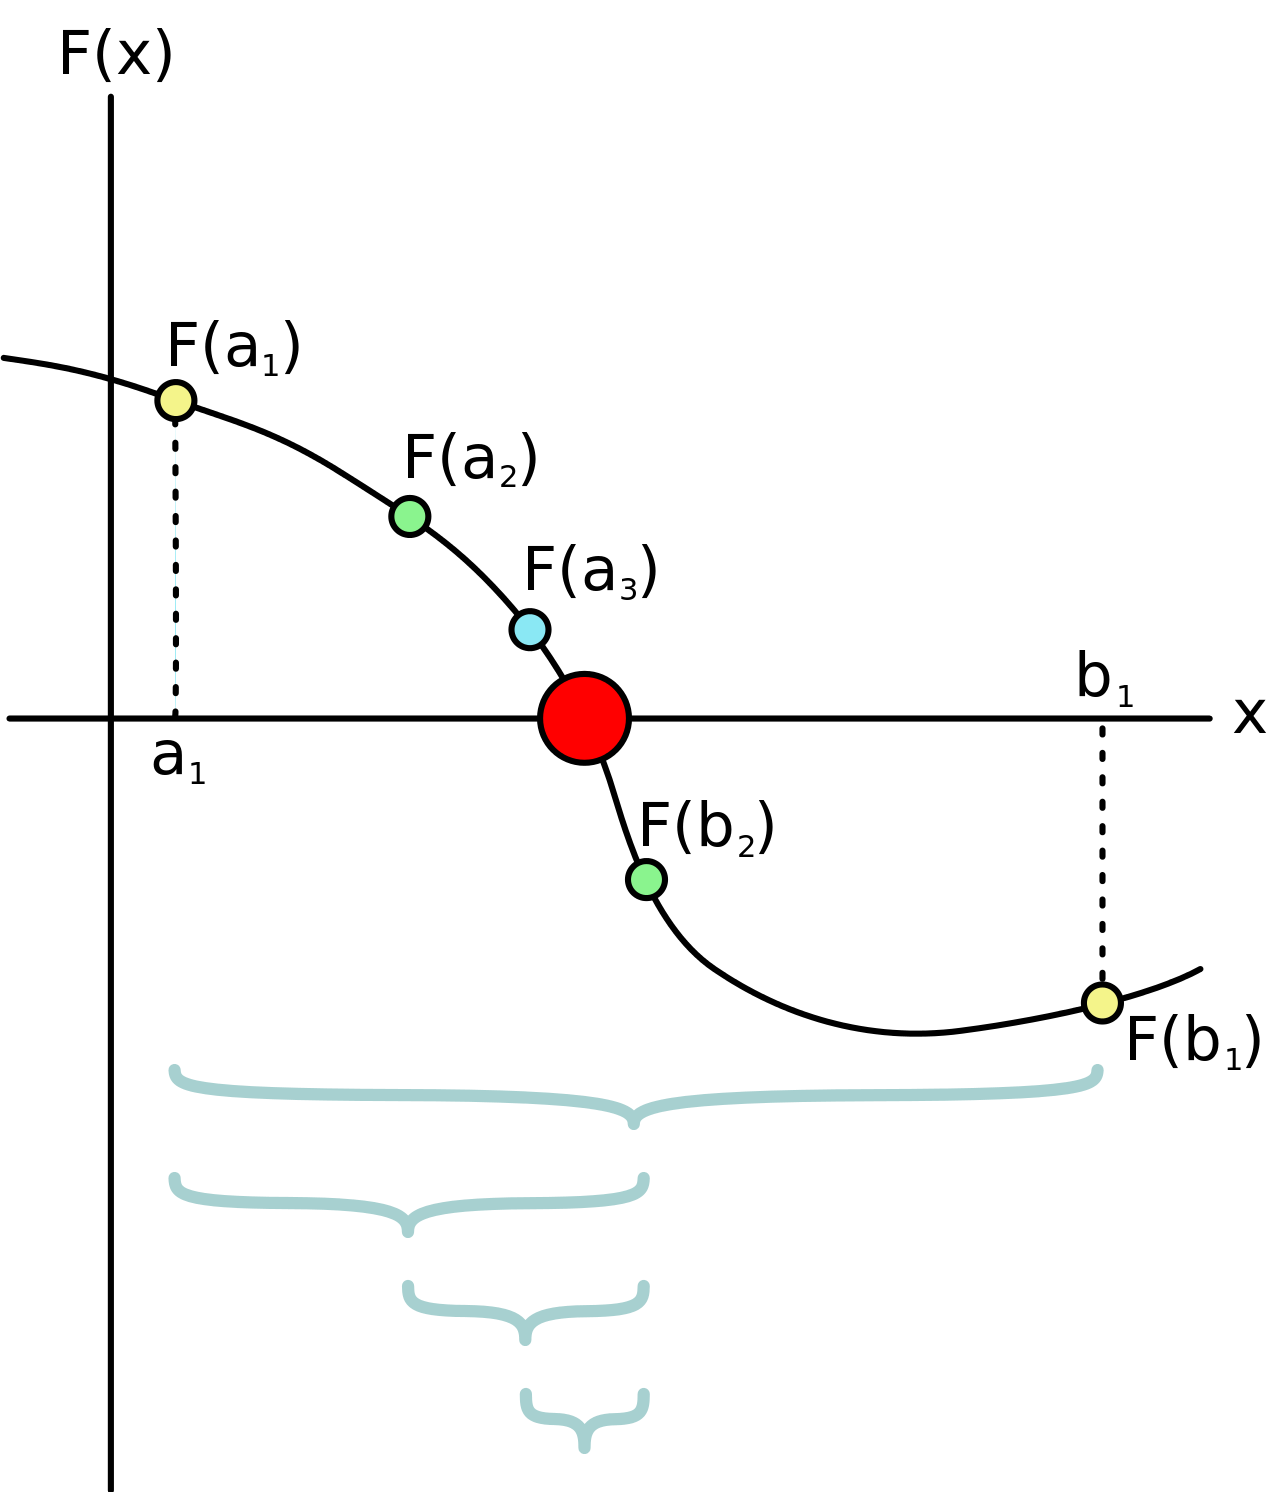
\includegraphics[width=0.75\textwidth]{plots/Bisection_method.png}
	\caption{Veranschaulichung einiger Iterationsschritte des Bisektionsverfahrens}
\end{figure}
\subsection*{Fixpunktverfahren}


\section*{Diagramme}
\subsection*{Benötigte Iterationen}
Es wurde jewiels die Funktion $g$ gewählt mit der das Fixpunktverfahren tatsächlich ein Ergebnis liefert (mehr dazu im Vergleich der Verfahren).

\begin{figure}[!h]
	\centering
	\begin{subfigure}[b]{0.4\textwidth}
		\caption*{$f_1(x) = x + e^x-2, g_{1,b}(x)=\log(2-x)$}
		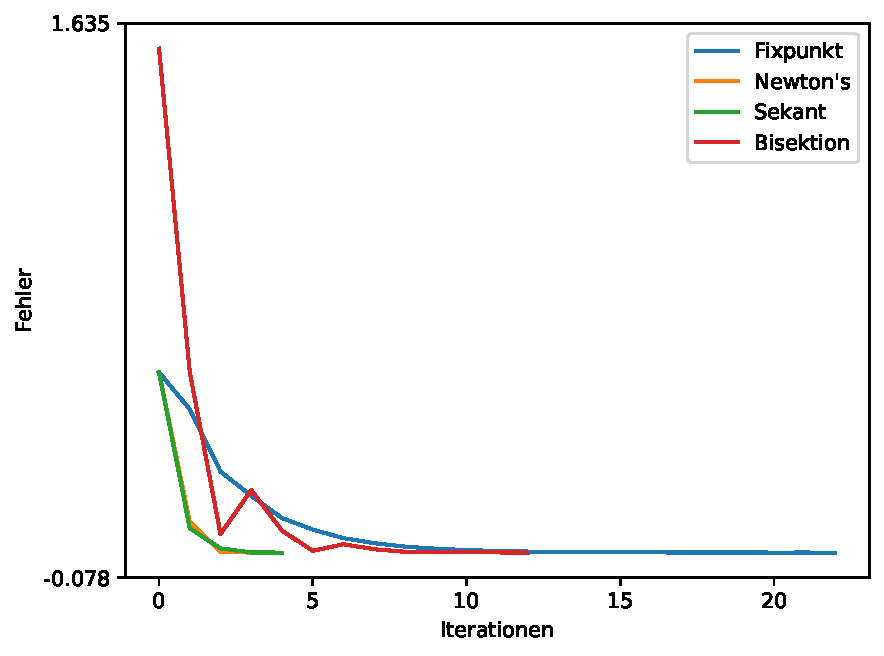
\includegraphics[width=\textwidth]{plots/plot.pdf}
	\end{subfigure}
	\begin{subfigure}[b]{0.4\textwidth}
		\caption*{$f_2(x) = 2x - \tan(x), g_{2,b}(x)=\arctan(2x)$}
		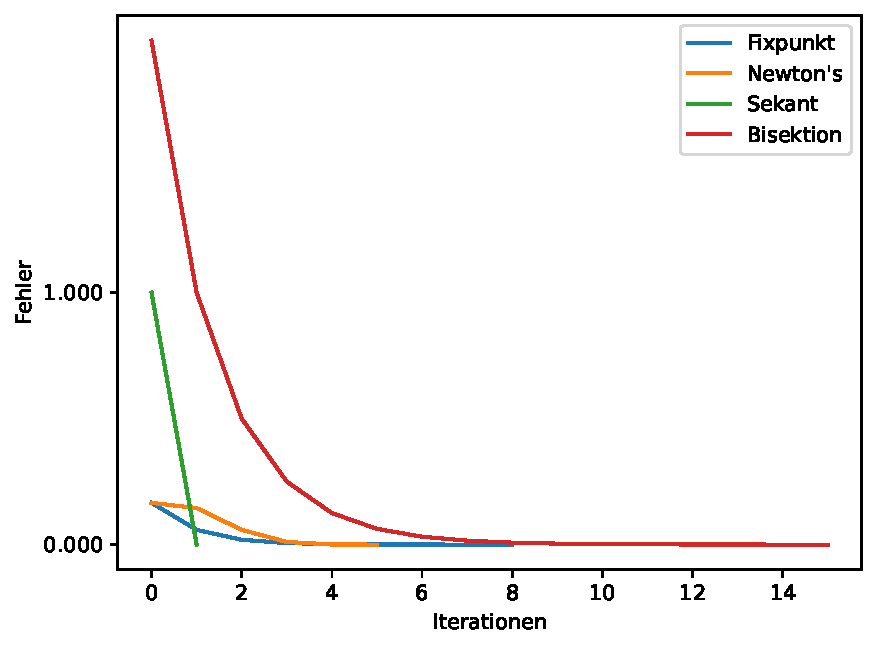
\includegraphics[width=\textwidth]{plots/plot1.pdf}
	\end{subfigure}
	\begin{subfigure}[b]{0.4\textwidth}
		\caption*{$f_{3,2}(x) = -2x^2 + 4$}
		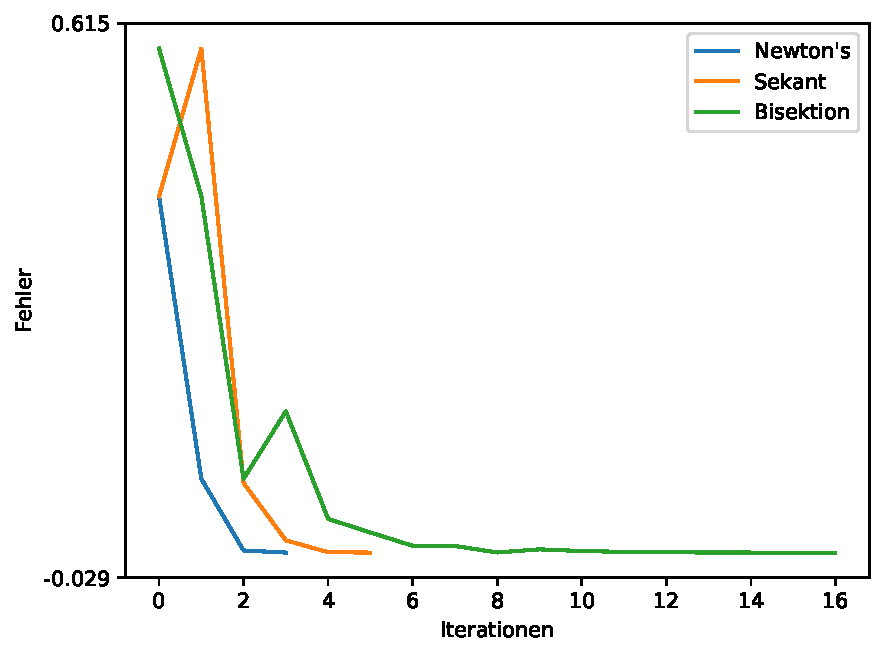
\includegraphics[width=\textwidth]{plots/plot2.pdf}
	\end{subfigure}
	\begin{subfigure}[b]{0.4\textwidth}
		\caption*{$f_{3,1}(x) = -x^2 + 2$}
		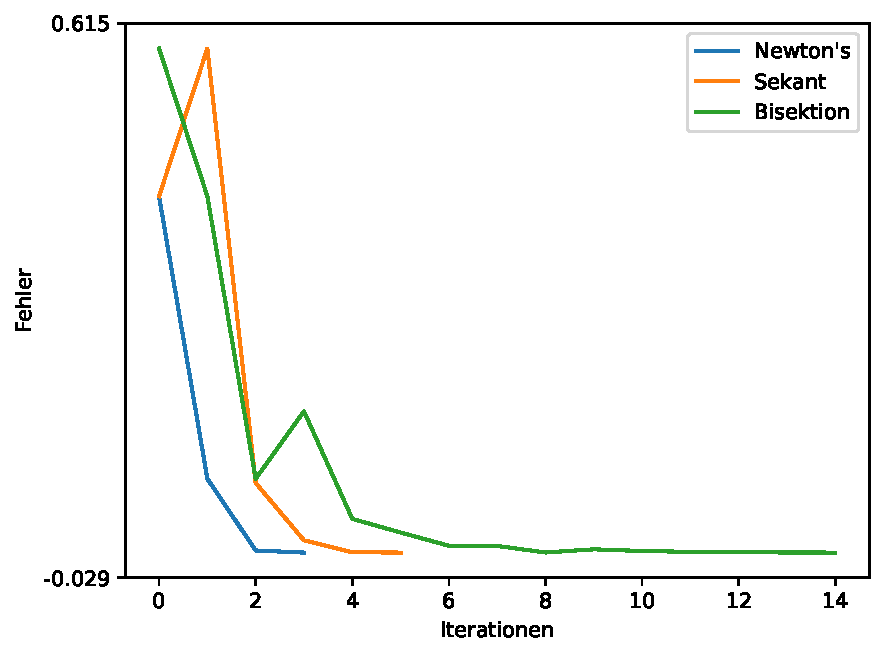
\includegraphics[width=\textwidth]{plots/plot3.pdf}
	\end{subfigure}
	\begin{subfigure}[b]{0.4\textwidth}
		\caption*{$f_{3,\frac{1}{4}}(x) = -\frac{1}{4}x^2 +\frac{1}{2},  g_{3,\frac{1}{4}}(x)=-\frac{1}{4}x^2 + x + \frac{1}{2}$}
		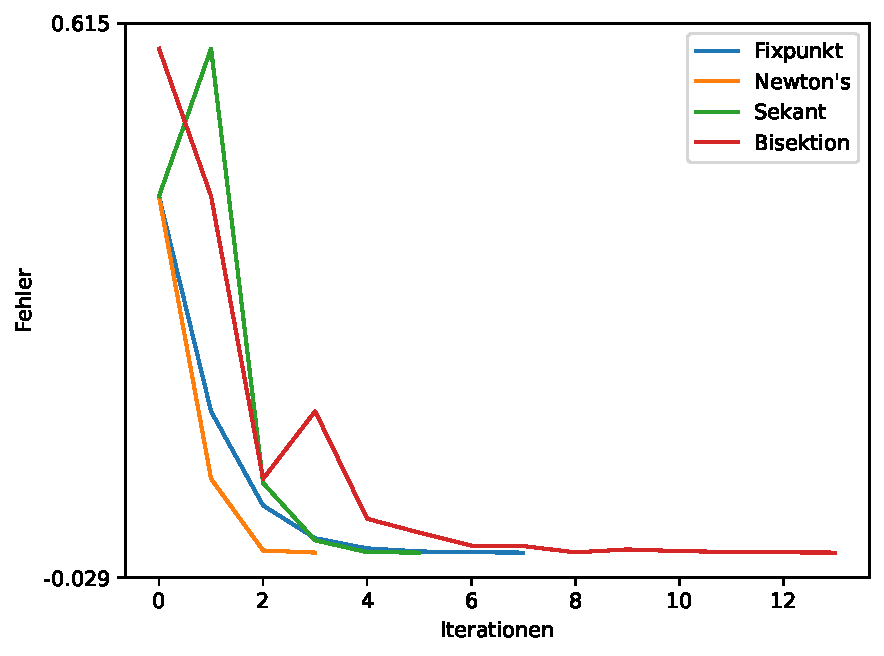
\includegraphics[width=\textwidth]{plots/plot4.pdf}
	\end{subfigure}
\end{figure}
\subsection*{Variation der Startwerte}
\section*{Vergleich der Verfahren}
Hier noch einige erhobene Daten zusammengefasst:
\begin{table}[!h]
	\centering
	\begin{tabular}{|c|c|c|c|c|} \hline
		                              & Newton & Sekanten & Bisektion & Fixpunkt \\ \hline
		Durchschnittliche Iterationen & 4.4    & 5        & 15        & 13.333   \\ \hline
		Maximale Iterationen          & 6      & 6        & 17        & 23       \\ \hline
	\end{tabular}
\end{table}

Beim betrachten dieser Daten ist zu beachten, dass lediglich 3 Datenpunkte zum Fixpunktverfahren existieren.
Stichpunkte:
Newton und Sekant klar am schnellsten, kleiner vorteil für newton evtl dadurch ausgeglichen, dass bei sekant nicht symbolisch differenziert werden muss
Fixpunkt funktioniert nur für geschickt gewählte funktionen (Kontraktion)
Für bisektion muss ungefähr bekannt sein wo die nullstelle liegt

\end{document}